% ==============================================================================
\subsection{Context}\label{aa:res:context}
\begin{figure}[h]
  \centering
  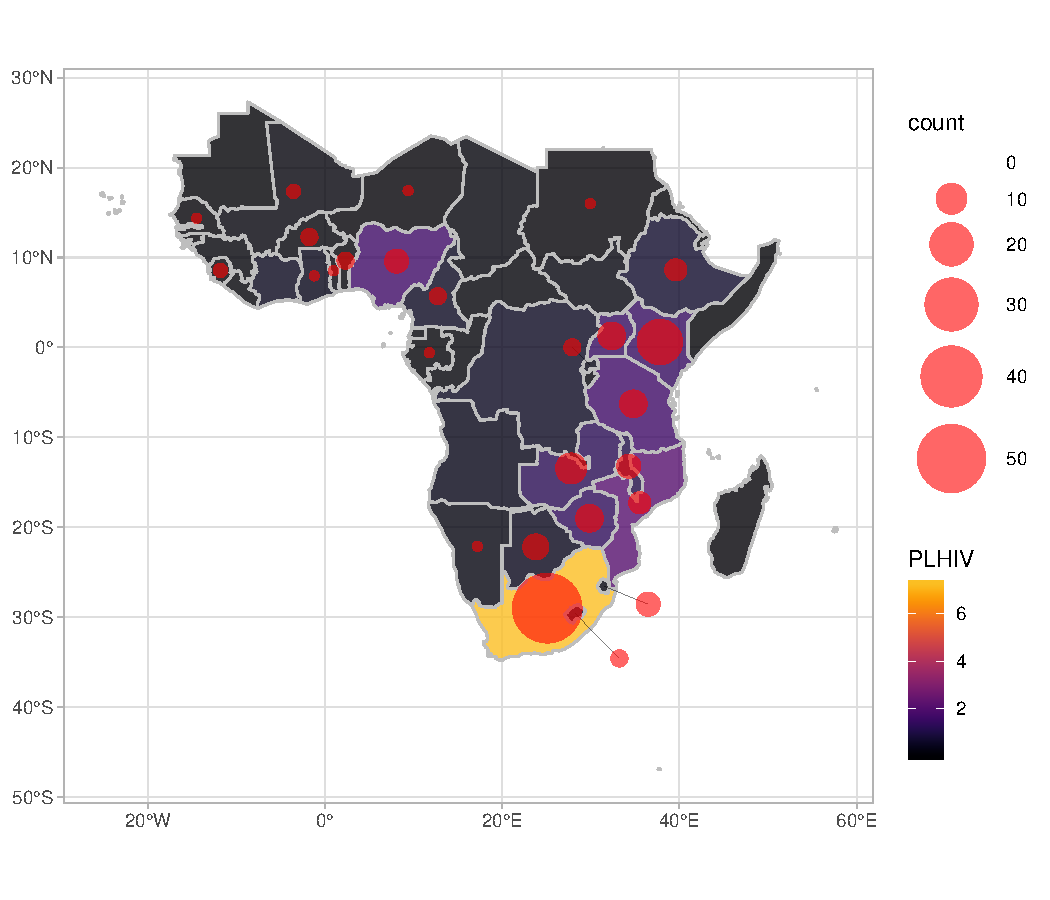
\includegraphics[width=0.8\linewidth]{map-n-vs-plhiv}
  \caption{Map showing number of studies (of \na total)
    applying HIV transmission modelling in each country vs
    the number of people living with HIV (PLHIV, millions)}
  \label{fig:map}
\end{figure}
% ==============================================================================
\subsection{Risk Heterogeneity}\label{aa:res:risk}
% ------------------------------------------------------------------------------
\subsubsection{Distributions}
\twocolumn
\filedef{\projectroot/out/tex/config/plot.list.dist}
\foreach \var/\title in \filedata{\hspace{0pt}%
  \begin{minipage}[t][.33\textheight][t]{\linewidth}
    \includegraphics[width=\linewidth]{{d.\var}.pdf}
    \captionof{figure}{\title}
    \label{fig:d:\var}
  \end{minipage}}
\onecolumn
\clearpage
% ==============================================================================
\subsection{ART Prevention Impact}\label{aa:res:api}
% ------------------------------------------------------------------------------
\subsubsection{Figures}
The following figures illustrate the projected ART prevention impact (Dataset~B),
stratified by various factors of heterogeneity and intervention conditions (colours).
The left panels show the relative reduction in HIV incidence rate;
the right panels show the relative reduction in cumulative new HIV infections;
both as compared to a base-case scenario reflecting status quo.
The number of studies (scenarios) reporting
incidence reduction, cumulative infections averted, both, or either was:
\x{n/n.a.api.inc}~(\x{n/n.s.api.inc}),
\x{n/n.a.api.chi}~(\x{n/n.s.api.chi}), 
\x{n/n.a.api.both}~(\x{n/n.s.api.both}), and
\x{n/n.a.api}~(\x{n/n.s.api}), respectively.
If any study included multiple scenarios of ART scale-up,
then each scenario was included separately,
but the size of each data point was reduced
in proportion to the number of scenarios;
so studies with only one scenario have the largest data points.
Some scenarios have multiple data points if multiple time horizons were reported.
If any factor could not be quantified due to missing data or varying values,
the data point is grey.
A small random offset has been added to the data points to reduce overlap.
\filedef{\projectroot/out/tex/config/plot.list.api}
\foreach \var/\title in \filedata{
  \begin{figure}[H]
    \begin{subfigure}{0.5\linewidth}
      \includegraphics[width=\linewidth]{{inc.s.\var}.pdf}
    \end{subfigure}%
    \begin{subfigure}{0.5\linewidth}
      \includegraphics[width=\linewidth]{{chi.s.\var}.pdf}
    \end{subfigure}
    \caption{\title}
    \label{fig:api:\var}
  \end{figure}
}
\begin{figure}[H]
  \begin{subfigure}{0.5\linewidth}
    \includegraphics[width=\linewidth]{{inc.s.Risk.both}.pdf}
    \caption{Reduction in HIV incidence (\%)}
  \end{subfigure}%
  \begin{subfigure}{0.5\linewidth}
    \includegraphics[width=\linewidth]{{chi.s.Risk.both}.pdf}
    \caption{Cumulative HIV infections averted (\%)}
  \end{subfigure}
  \caption{Projected ART prevention benefits,
    stratified by factors of risk heterogeneity: whether models considered
    differences in sexual activity, key populations, and
    ART cascade prioritized to key populations.
    Subset of studies reporting both outcomes.}
  \label{fig:api:both}
\end{figure}
% ------------------------------------------------------------------------------
\subsubsection{Table}
Table~\ref{tab:api} summarizes the median [IQR] projected ART prevention impact (Dataset~B),
stratified by various factors of heterogeneity and intervention conditions.
Reported p-values for each factor are from non-parametric Kruskal-Wallis tests
for differences in ART prevention impact under at least one of the factor levels.
\begin{table}[H]
  \caption{Projected ART prevention benefits,
    stratified by factors of risk heterogeneity and conditions of ART scale-up}
  \centering
  \newcommand{\xtab}[1]{\x{api/inc/#1.xtab} & \x{api/chi/#1.xtab} }%
\def\baselinestretch{1.1}\footnotesize%
\centerline{%
\setlength{\tabcolsep}{.7ex}%
\begin{tabular}{ll rrc rc rrc rc}
  \toprule
  & & \multicolumn{5}{c}{Incidence Reduction (\%)}
    & \multicolumn{5}{c}{Cumulative Infections Averted (\%)} \\
  \cmidrule(rl){3-7}\cmidrule(rl){8-12}
  Factor               & Level            & N\tn{a} & Median & (IQR) & Effect\tn{b} & (95\% CI)\tn{b} 
                                          & N\tn{a} & Median & (IQR) & Effect\tn{b} & (95\% CI)\tn{b} \\
  \midrule
%%\begin{tabular}{lll}
  Time Horizon         & 0-10             & \xtab{t.cat.0}               \\
  (years)              & 11-20            & \xtab{t.cat.10}              \\
                       & 21-30            & \xtab{t.cat.20}              \\
                       & 31+              & \xtab{t.cat.30}              \\[\tsep]
  HIV Prevalence       & 10+              & \xtab{api.prev.cat.High}     \\
  (\%)                 & 1-10             & \xtab{api.prev.cat.Mid}      \\
                       & 0-1              & \xtab{api.prev.cat.Low}      \\[\tsep]
  HIV Incidence        & Increasing       & \xtab{api.phase.incr}        \\
  Trend\tn{c}          & Inc-to-stable    & \xtab{api.phase.its}         \\
                       & Stable           & \xtab{api.phase.stab}        \\
                       & Dec-to-stable    & \xtab{api.phase.dts}         \\
                       & Decreasing       & \xtab{api.phase.decr}        \\
  \midrule
  RR Transmission      & 0.0-0.039        & \xtab{art.rbeta.cat.0}       \\
  on ART               & 0.04-0.099       & \xtab{art.rbeta.cat.0.04}    \\
                       & 0.1+             & \xtab{art.rbeta.cat.0.1}     \\[\tsep]
  CD4 Threshold for    & Symptomatic      & \xtab{art.cd4.symp}          \\
  ART Initiation       & 200              & \xtab{art.cd4.200}           \\
                       & 350              & \xtab{art.cd4.350}           \\
                       & 500              & \xtab{art.cd4.500}           \\
                       & Any              & \xtab{art.cd4.All}           \\
                       & Mixed            & \xtab{art.cd4.*}             \\[\tsep]
  ART Coverage         & 0-59             & \xtab{art.cov.cat.0}         \\
  Target (\%)\tn{c}    & 60-84            & \xtab{art.cov.cat.0.6}       \\
                       & 85+              & \xtab{art.cov.cat.0.85}      \\
  \midrule
  Acute Infection      & No               & \xtab{hiv.x.acute.FALSE}     \\
                       & Yes              & \xtab{hiv.x.acute.TRUE}      \\[\tsep]
  Late-Stage Infection & No               & \xtab{hiv.x.late.FALSE}      \\
                       & Yes              & \xtab{hiv.x.late.TRUE}       \\[\tsep]
  Trans. Drug Resist.  & No               & \xtab{art.tdr.FALSE}         \\
                       & Yes              & \xtab{art.tdr.TRUE}          \\
  \midrule
  HIV Morbidity        & No               & \xtab{hiv.morb.any.FALSE}    \\
                       & Any              & \xtab{hiv.morb.any.TRUE}     \\[\tsep]
  HTC Behav. Change    & No               & \xtab{bc.any.FALSE}          \\
                       & Any              & \xtab{bc.any.TRUE}           \\
  \midrule
  Risk Definition      & None             & \xtab{Risk.None}             \\
                       & Activity (No KP) & \xtab{Risk.Activity-(no-KP)} \\
                       & KP (Priority)    & \xtab{Risk.KP-(priority)}    \\
                       & KP (Same)        & \xtab{Risk.KP-(same)}        \\[\tsep]
  Activity Turnover    & No               & \xtab{act.turn.any.FALSE}    \\
                       & Yes              & \xtab{act.turn.any.TRUE}     \\[\tsep]
  Partnership Types    & Generic          & \xtab{pt.def.gen}            \\
                       & By Groups        & \xtab{pt.def.grp}            \\
                       & Overlapping      & \xtab{pt.def.phen}           \\[\tsep]
  Sex Stratification   & No               & \xtab{act.def.sex.FALSE}     \\
                       & Yes              & \xtab{act.def.sex.TRUE}      \\
  \bottomrule
\end{tabular}}
\floatfoot{
  \tnt[a]{N: number of unique scenarios and time horizons;
    sums across factor levels may be less than 126 and 115 due to missing variables.}
  \tnt[b]{Effect estimates from linear multivariate regression
    with generalized estimating equations \cite{Hojsgaard2006};
    effects are illustrated in Figure~\ref{fig:effects}.}
  \tnt[c]{Omitted from regression model due to missing data.}
  RR: relative risk;
  HTC: HIV testing and counselling;
  KP: key populations.
  priority: modelled ART cascade transitions were faster in KP vs overall due to prioritized programs;
  same: cascade transitions were assumed the same in KP as overall.
  Factor definitions are given in Appendix~\ref{a:defs}.
}

  \label{tab:api}
\end{table}